\documentclass[12pt, letter]{report}

\usepackage{amsmath}    % need for subequations
\usepackage[pdftex]{graphicx}   % need for figures
\usepackage{verbatim}   % useful for program listings
\usepackage{color}      % use if color is used in text
\usepackage{caption}  
\usepackage{subcaption}  % use for side-by-side figures
\usepackage{hyperref}   % use for hypertext links, including those to external documents and URLs
\usepackage{cleveref}
\usepackage{setspace}
\doublespacing

\allowdisplaybreaks
\captionsetup{compatibility=false}

\graphicspath{{fluid_figs/}}


\begin{document}

\chapter{Fluid Mechanics and Acoustics Background}
\section{Conservation Laws}
It is my goal for thesis to be accessible to researchers who are not experts in fluid dynamics. In addition, I also want to emphasize the time domain model of later chapters is as much a derivation from first principles as possible. So in this chapter we will review some important concepts and results from fluid dynamics and acoustics, which we will use later on in deriving a description of the rat vocal tract. Discussions similar to these can be found in Batchelor \cite{Batchelor2000} and Howe \cite{howe2003theory}. 

The state of a fluid at time t and position $\textbf{x}$ is determined by its velocity field $\textbf{v}(\textbf{x}, t)$ and any two thermodynamic variables. Common choices for these thermodynamic variables are the pressure field $p(\textbf{x}, t)$, density field $\rho(\textbf{x}, t)$, or temperature field $T(\textbf{x}, t)$. We thus need five scalar equations to specify the equations of motion for the fluid.

\subsection{Mass Conservation}
The first equation of motion is a statement of conservation of mass. To derive it we consider the total mass in a volume $V$, which can be expressed as a volume integral of the fluid density
\begin{equation}
\label{eq:mass}
M = \int_V \rho dV.
\end{equation}
If we consider an infinitesimal element $d\textbf{S}$ of the volume's enclosing surface $S$, the net flux of mass through that infinitesimal element is $\rho \textbf{v} \cdot d\textbf{S}$. Thus the total flux of mass through $S$ is given by the surface integral of that quantity.
\begin{equation}
\label{eq:flux}
\Phi_M = \int_S \rho \textbf{v} \cdot d\textbf{S}.
\end{equation}
Conservation of mass states that the time rate of change of the mass in $V$ plus the net flux through $S$ must equal $0$.
\begin{equation}
\label{eq:conservation1}
\frac{d M}{d t} + \Phi_M = 0
\end{equation}
Substituting Eqs. \ref{eq:mass} and \ref{eq:flux} into \ref{eq:conservation1} we get
\begin{equation}
\int_V \frac{\partial \rho}{\partial t} dV + \int_S \rho \textbf{v} \cdot d\textbf{S} = 0.
\end{equation}
Now using the divergence theorem on the second integral we can express this equation as
\begin{equation}
\int_V \left(\frac{\partial \rho}{\partial t} + \nabla \cdot \left( \rho \textbf{v} \right)\right) dV = 0.
\end{equation}
This equation must be true for all volumes $V$. Thus, the integrand must be equal to $0$, and we obtain the equation of fluid continuity \cite{Batchelor2000}.
\begin{equation}
\label{eq:continuity}
\frac{\partial \rho}{\partial t} + \nabla \cdot \left( \rho \textbf{v} \right)=0.
\end{equation}

\subsection{Energy Conservation}
For general fluid dynamics problems, especially ones in which there is significant heat conduction due to temperature gradients, the full energy transport equation must be used to describe the spatial and temporal evolution of energy distributions in the system. However, we are mostly concerned with the flow of air in the rodent vocal tract. Rats complete a full respiration cycle approximately eight times per second. Thus, it is not a bad approximation to neglect heat conduction and assume the air remains at room temperature. This assumption simplifies the energy analysis greatly. By neglecting heat conduction it can be assumed that the the fluid is homentropic, meaning the fluid's specific entropy $s$ is constant and uniform. This allows the assumption that the fluid's pressure and density are related by a constitutive equation of the form
\begin{equation}
\label{eq:constitutive}
p = p(\rho, s).
\end{equation}
Often times simply assuming the fluid to be an ideal gas is sufficient. The constitutive equation for an adiabatic ideal gas is
\begin{equation}
p = constant \times \rho^\gamma,
\end{equation}
where $\gamma$ is the ratio of specific heats of the gas. For our purposes we will be able to use an even simpler relation. Since we are mainly interested in the production of sound, we will be able to use the fact that acoustic flow consists of small perturbations from a mean flow to derive a constitutive equation. This relation is discussed more in the section on acoustic flow \cite{howe2003theory}. 
\subsection{Momentum Conservation}
The momentum conservation equation comes from similar considerations as the previous section. We will derive an expression for the net momentum in a volume $V$ and relate its time rate of change to the net flux of momentum through the volume's enclosing surface $S$. Although this process will be made somewhat more complicated by the fact that momentum is a vector quantity. The $i^{th}$ component of the total linear momentum in volume $V$ is given by
\begin{equation}
\label{eq:momentum}
P_i = \int_V \rho v_i dV
\end{equation}
Furthermore the rate at which momentum flows through infinitesimal area $d\textbf{S}$ is given by $\rho \textbf{v} (\textbf{v} \cdot d\textbf{S})$. Thus, the total flux of the $i^{th}$ momentum component through $S$ is given by.
\begin{equation}
\label{eq:momentum_flux}
\Phi_i = \int_S \rho v_i v_j dS_j,
\end{equation}
where summations are carried out over repeated indices. Finally, we will need an expression for the net force on $V$. The $i^{th}$ component of that force is given by
\begin{equation} 
\label{eq:force}
f_i = \int_V F_i dV + \int_S \sigma_{ij} dS_j,
\end{equation}
where the left integral is the total contribution from body forces, such as gravity. The right integral is the total contribution from surface forces, such as those arising in shear flow. The matrix $sigma_{ij}$ is the stress tensor. Conservation of momentum and Newton's second law states that the time rate of change of momentum inside $V$ plus the flux of momentum through $S$ must equal the net force on $V$.
\begin{equation}
\label{eq:momentum_conservation1}
\frac{d P_i}{d t} + \Phi_i = f_i.
\end{equation}
Inserting Eqs. \ref{eq:momentum}, \ref{eq:momentum_flux}, and \ref{eq:force} into Eq. \ref{eq:momentum_conservation} we get
\begin{equation}
\int_V \frac{\partial \rho v_i}{\partial t} dV + \int_S \rho v_i v_j dS_j = \int_V F_i dV + \int_S \sigma_{ij} dS_j.
\end{equation}
Now we can use the divergence theorem to convert the surface integrals into volume integrals.
\begin{equation}
\int_V \left( \frac{\partial \rho v_i}{\partial t} + \frac{\partial (\rho v_i v_j)}{\partial x} \right) dV = \int_V \left( F_i + \frac{\partial \sigma_{ij}}{\partial x} \right) dV.
\end{equation}
Again this equation must be valid for arbitrary volumes $V$, so we can set the integrands equal to each other.
\begin{equation}
\frac{\partial \rho v_i}{\partial t} + \frac{\partial (\rho v_i v_j)}{\partial x} = F_i + \frac{\partial \sigma_{ij}}{\partial x}.
\end{equation}
Expanding the derivatives and rearranging the terms of this equation we get
\begin{equation}
\left( \frac{\partial \rho}{\partial t} + v_j \frac{\partial \rho}{\partial x_j} + \rho \frac{\partial v_j}{\partial x_j} \right) v_i + \rho \left( \frac{\partial v_i}{\partial t} + v_j \frac{\partial v_i}{\partial x_j} \right) = F_i + \frac{\partial \sigma_{ij}}{\partial x_j}.
\end{equation}
Now combining it with the continuity equation in tensor form,
\begin{equation}
\frac{\partial \rho}{\partial t} + v_j \frac{\partial \rho}{\partial x_j} + \rho \frac{\partial v_j}{\partial x_j} = 0,
\end{equation}
we can eliminate the derivatives of density and obtain the equation of fluid motion.
\begin{equation}
\rho \left( \frac{\partial v_i}{\partial t} + v_j \frac{\partial v_i}{\partial x_j} \right) = F_i + \frac{\partial \sigma_{ij}}{\partial x_j}.
\end{equation}
This can be expressed as
\begin{equation}
\label{eq:momentum_transport}
\frac{D v_i}{\partial t} = \frac{F_i}{\rho} + \frac{1}{\rho}\frac{\partial \sigma_{ij}}{\partial x_j},
\end{equation}
where 
\begin{equation}
\frac{D}{Dt} = \frac{\partial }{\partial t} + v_j \frac{\partial }{\partial x_j}
\end{equation}
is known as the convective derivative \cite{Batchelor2000}. 

\section{The Stress Tensor}
\subsection{Symmetry of the Stress Tensor}
In this subsection we will derive an expression for the torque on a fluid of volume $V$ to show that the stress tensor must be symmetric. The $i^{th}$ component of the torque about the origin $O$ from a body force on an infinitesimal volume element $dV$ inside of $V$ is $\varepsilon_{ijk} x_j F_k dV$. Similarly the $i^{th}$ component of torque on an infinitesimal area element $d\textbf{S}$ of the surface $S$ is $\varepsilon_{ijk} x_j \sigma_{kl} dS_l$. In these expressions $\varepsilon_{ijk}$ is the Levi-Civita tensor and is defined by
\begin{equation}
\varepsilon_{ijk} =
\begin{cases}
1 & \text{i,j,k is an even permutation of 1,2,3} \\
-1 & \text{i,j,k is an odd permutation of 1,2,3} \\
0 & \text{otherwise}
\end{cases}
\end{equation}
Integrating the first expression over $V$ and the second over $S$ we get an expression for the total torque on $V$ about $O$.
\begin{equation}
\tau_i = \int_V \varepsilon_{ijk} x_j F_k dV + \int_S \varepsilon_{ijk} x_j \sigma_{kl} dS_l.
\end{equation}
Using the divergence theorem to turn the area integral into a volume integral,
\begin{equation}
\tau_i = \int_V \varepsilon_{ijk} x_j F_k dV + \int_V \varepsilon_{ijk} \frac{\partial (x_j \sigma_{kl})}{\partial x_l} dV.
\end{equation}
Now expanding the derivative in the second integral, this becomes
\begin{equation}
\tau_i = \int_V \varepsilon_{ijk} x_j F_k dV + \int_V \varepsilon_{ijk} \sigma_{kj} dV + \int_V \varepsilon_{ijk} x_j\frac{\partial \sigma_{kl}}{\partial x_l}dV.
\end{equation}
Now we consider the case in which the point $O$ lies within $V$ and we allow the volume to tend to $0$. If the volume is sufficiently small, then $F_i$, $\sigma_{ij}$, and $\frac{\partial \sigma_{ij}}{\partial x_j}$ will not vary significantly over the region of integration. From this we can conclude the first, second, and third integrals in the above equation will scale as $V^{4/3}$, $V$, and $V^{4/3}$ respectively (since $x_j ~ V^{1/3}$). From Newton's second law for rotational motion we know the time rate of change of angular momentum of the fluid volume must equal the torque applied to it. However, we also know that the rate of change of angular momentum should scale as $V^{4/3}$, since the net linear acceleration scales as $V$, and the rate of change of angular momentum scales as $xV$. This is inconsistent with our above result, which shows that the rate of change of angular momentum will be dominated by the second integral in the above equation, since it scales as $V$. The only way to resolve this inconsistency is for the second integral to be identically $0$ for all choices of $O$ and $V$. This is only possibly if
\begin{equation}
\varepsilon_{ijk} \sigma_{kj} = 0,
\end{equation}
which implies that stress tensor must be symmetric \cite{Batchelor2000}
\begin{equation}
\sigma_{ij} = \sigma_{ji}.
\end{equation}
\subsection{The Stress Tensor in a Static Fluid}
It is a well known result from linear algebra that a symmetric matrix can be diagonalized by expressing its entries in a rotated coordinate system. The axes of this coordinate system are called the principle axes. Thus from the result of the previous section we can choose a set of principle axes to diagonalize the stress tensor at a single point in space. Let's call the diagonal elements of the rotated stress tensor $\sigma^{'}_{11}$, $\sigma^{'}_{22}$, and $\sigma^{'}_{33}$. It is another well known result from linear algebra that the sum of the diagonals of a matrix is invariant under a change of basis. Thus the trace of the stress tensor at the point in space can be expressed as
\begin{equation}
\sigma_{ii} = \sigma^{'}_{11} + \sigma^{'}_{22} + \sigma^{'}_{33},
\end{equation}
regardless of the chosen basis.

Now let's consider the surface forces acting on an infinitesimal cubic volume in a static fluid. The cube is small enough such that the entries of the stress do not vary significantly throughout its volume. We can also choose the cube so its sides are aligned parallel to the principle axes of the stress tensor, which will ensure its off diagonal elements are $0$. We can then express the stress tensor as the sum of two matrices.
\begin{equation}
\boldsymbol{\sigma}=
\begin{pmatrix}
\frac{\sigma_{ii}}{3} & 0 & 0 \\
0 & \frac{\sigma_{ii}}{3} & 0 \\
0 & 0 & \frac{\sigma_{ii}}{3}
\end{pmatrix}
+
\begin{pmatrix}
\sigma^{'}_{11}-\frac{\sigma_{ii}}{3} & 0 & 0 \\
0 & \sigma^{'}_{22}-\frac{\sigma_{ii}}{3} & 0 \\
0 & 0 & \sigma^{'}_{33}-\frac{\sigma_{ii}}{3}
\end{pmatrix}
\end{equation}
By construction $Tr(\boldsymbol{\sigma})=\sigma_{ii}$, which also equals the trace of the first matrix on the right hand side. Thus the trace of second matrix must be $0$. From that we can conclude that there are forces compressing the fluid volume in the direction of two principle axes and one force tensioning the fluid volume in the direction of the other axis. This force distribution has the tendency to elongate and deform the volume. These forces cannot be balanced out by internal volume forces, since volume forces tend to $0$ faster than surfaces as we let the volume go to $0$. This presents an inconsistency, since a fluid is defined as a material that is incapable of withstanding a tendency of applied forces to change its shape. It follows that the diagonal components of the second matrix must all be $0$. Therefore the principle stresses must all be equal to $\frac{\sigma_{ii}}{3}$. We can define $p=-\frac{\sigma_{ii}}{3}$, which is called the static fluid pressure. Thus,
\begin{equation}
\sigma_{ij} = -p \delta_{ij}.
\end{equation}
The stress tensor in a static fluid then has the interpretation of isotropically compressing all fluid volumes with force per unit area equal to the static pressure \cite{Batchelor2000}.

\subsection{The Stress Tensor in a Moving Fluid}
In a moving fluid there a shear forces in addition the normal forces from the static pressure. To account for these shear forces we express the stress tensor as the sum of the static fluid part and a non-isotropic which accounts for shear forces that arise from the fluid motion.
\begin{equation} 
\label{eq:stress}
\sigma_{ij} = -p \delta_{ij} + d_{ij}
\end{equation}
The tensor $d_{ij}$ is called the deviatoric stress tensor. It is symmetric, since $\sigma_{ij}$ must be symmetric. In addition, it has trace equal to $0$, since the trace of $\boldsymbol{\sigma}$ must equal the sum of the normal stresses. Furthermore, the deviatoric stress cannot depend on the absolute velocity of the fluid. Since for a fluid traveling at constant velocity we can always change our inertial frame of reference to one comoving with the fluid, and this transformation should not affect the stresses present in the fluid. Therefore, it is reasonable to assume $d_{ij}$ depends on gradients of fluid velocity. The simplest assumption for such a tensor is one for which it is a linear function of the velocity gradients. 
\begin{equation} 
d_{ij} = A_{ijkl} \frac{\partial v_k}{\partial x_l}.
\end{equation}
Fluids that obey such a tensor are known as Newtonian fluids. Although many fluids deviate from this assumption it will be more than sufficient for our purposes. It is also common to assume the fluid is isotropic, meaning the fluid has the same properties in all directions. For an isotropic fluid it is reasonable to expect the fourth order tensor $A_{ijkl}$ is isotropic. Thus any anisotropy in $d_{ij}$ is a result of the velocity gradients. The most general expression for an isotropic fourth order tensor is 
\begin{equation}
A_{ijkl} = \mu \delta_{ij}\delta_{kl} + \mu^{'} \delta_{ik}\delta_{jl} + \mu^{''} \delta_{il}\delta_{jk}
\end{equation}
Thus,
\begin{equation}
d_{ij} = \mu \frac{\partial v_k}{\partial x_k} + \mu^{'} \frac{\partial v_i}{\partial x_j}+\mu^{''} \frac{\partial v_j}{\partial x_i} 
\end{equation}
However, $d_{ij}$ must also be symmetric and traceless which means $\mu^{'}=\mu^{''}$ and $3\mu = -2\mu^{'}$. Therefore we can finally express the stress tensor as
\begin{equation}
\label{eq:deviatoric}
d_{ij} = 2 \mu \left( e_{ij}- \frac{1}{3} e_{kk}\delta_{ij} \right),
\end{equation}
where
\begin{equation}
\label{eq:rate_of_strain}
e_{ij}=\frac{1}{2}\left( \frac{\partial v_i}{\partial x_k} + \frac{\partial v_j}{\partial x_i} \right).
\end{equation}
The quantity $e_{ij}$ is known as the rate of strain tensor and the quantity $\mu$ has the interpretation of being the viscosity of the fluid \cite{Batchelor2000}.

\section{The Navier-Stokes and Euler Equations}
The momentum transport equation can be used in combination with the expression for the stress tensor in terms of the velocity gradients to obtain the equation of motion for a isotropic, Newtonian, classical fluid. Combining Eqs. \ref{eq:momentum_transport}, \ref{eq:stress}, \ref{eq:deviatoric}, and \ref{eq:rate_of_strain} we get
\begin{equation}   
\rho \frac{D v_i}{D t} = F_i - \frac{\partial p}{\partial x_i} + \mu \left( \frac{\partial^2 v_i}{\partial x_j^2} + \frac{1}{3} \frac{\partial^2 v_j}{\partial x_i x_j}\right).
\end{equation}
Writing this in vector form it becomes
\begin{equation}
\label{eq:navier} 
\rho \frac{D \textbf{v}}{D t} = \textbf{F} - \nabla p + \mu \left( \nabla^2 \textbf{v} + \frac{1}{3} \nabla (\nabla \cdot \textbf{v})\right).
\end{equation}
This is the Navier-Stokes equation \cite{Batchelor2000}. Its three components, along with the continuity equation (Eq. \ref{eq:continuity}), and a constitutive equation of the form Eq. \ref{eq:constitutive} give the five equations of motion necessary to solve for the three velocity components $v_i$, the pressure $p$, and the density $\rho$ for Newtonian homentropic flow in an isotropic fluid. In general this is a very difficult task and much work is done performing direct numerical simulations of these equations. In practice it is generally not necessary to use the equations of motion in their full form, and additional simplifying assumptions can be introduced. In the following sections I will discuss the special types of flow I have used to model the acoustics of the rat vocal tract.

The first simplifying assumption is the neglecting of viscosity. In the Navier-Stokes equation, for flows with Reynold's numbers much greater than unity, the inertial terms become much greater than viscous terms. This allows one to neglect viscosity. The rat vocal folds have a radius of approximately $r=1$ mm, and the flow them has velocities on the order $U=30 \frac{m}{s}$. Thus the Reynold's number, $Re=\frac{r U}{\nu}$, (where $\nu$ is the kinematic viscosity of air) of this flow is on the order of $2000$. Therefore we will neglect viscosity in much of the analysis of this flow. The equation of motion for inviscid flow is called the Euler equation \cite{Batchelor2000}.
\begin{equation}
\label{eq:euler} 
\rho \frac{D \textbf{v}}{D t} = \textbf{F} - \nabla p.
\end{equation} 


\section{Linear Acoustic Flow}
\subsection{The Acoustic Wave Equation}
This type of flow models the propagation of sound in an inviscid fluid. In later chapters, we will use this type of flow to model the the acoustics of the rodent upper vocal tract. The linear nature of this flow comes from the fact that only small fluctuation from a quasi-steady mean flow. The intensity of sound pressure in air is measured using a decibel scale. The decibel value of a sound is calculated using the expression
\begin{equation}
20 log_{10} \left( \frac{|p|}{p_{ref}} \right),
\end{equation}
where the reference pressure $p_ref=2 \times 10^{-5} \frac{N}{m^2}$. An acoustic perturbation of $p=1 atm$ has an intensity of about $194$ dB, which is deafening. 

The pressure, density, and velocity can be written as the sum of a mean and small fluctuating component. $p=p_0 + p^{'}$, $v=v_0 + v^{'}$, $\rho=\rho_0 + \rho^{'}$. Now substituting these assumptions into Eqs. \ref{eq:euler} and \ref{eq:continuity},
\begin{equation}
\label{eq:linear1}
\begin{split}
\rho_0 \frac{\partial \textbf{v}^{'}}{\partial t} + \nabla p^{'} &= \textbf{F} \\
\frac{1}{\rho_0}\frac{\partial \rho^{'}}{\partial t} + \nabla \cdot \textbf{v}^{'} = q,
\end{split}
\end{equation}
In this step products of primed quantities have been neglected. Since $\frac{v^{'}}{v_0} \ll 1$, $\frac{p^{'}}{p_0} \ll 1$, and $\frac{\rho^{;'}}{\rho_0} \ll 1$ the products of primed quantities will be even smaller and can be safely neglected. In addition, the fact that mean quantities must also satisfy the equations of motion has been used. The equations for the mean quantities have been subtracted off from the equations for the full quantities. Lastly, a volume source term $q$ has been introduced into the continuity equation to account for changes in fluid volume, which can be a source of sound. Eliminating $\textbf{v}^{'}$ between the linearized momentum and continuity equations,
\begin{equation}
\label{eq:linear2}
\frac{\partial^2 \rho^{'}}{\partial t^2} - \nabla^2 p^{'} = \rho_0 \frac{\partial q}{\partial t} - \nabla \cdot \textbf{F}.
\end{equation}

Now a constitutive relation between $p^{'}$ and $\rho^{'}$ is needed. This relation for the undisturbed and disturbed states can be written
\begin{equation}
\begin{split}
p_0 &= p(\rho_0, s) \\
p_0 + p^{'} = p(\rho_0+\rho^{'},s) \approx p(p_0, s) + \left( \frac{\partial p}{\partial \rho}(\rho,s) \right)_0 \rho^{'}.
\end{split}
\end{equation}
The derivative in parentheses has dimensions of velocity squared and has the interpretation of being the square speed of sound in the medium $c$. Inserting this interpretation into the above equations and using the first equation to eliminate $p_0$ and $p(p_0, s)$ from the second equation we get a relationship between $ p^{'}$ and $\rho^{'}$.
\begin{equation} 
p^{'} = c^2 \rho^{'}.
\end{equation}
Using this equation to eliminate $\rho^{'}$ from Eq. \ref{eq:linear2} we get the acoustic wave equation for pressure perturbations driven by volume sources $q$ and body forces $\textbf{F}$.
\begin{equation} 
\label{eq:pressure_wave}
\left( \frac{1}{c^2}\frac{\partial^2 }{\partial t^2} - \nabla^2 \right)p^{'}=\rho_0 \frac{\partial q}{\partial t} - \nabla \cdot \textbf{F}
\end{equation}

If there are no body forces (i.e. $\textbf{F}=0$), then Eq. \ref{eq:linear1} implies the existence of a velocity potential $\phi^{'}$ such that
\begin{equation}
\label{eq:velocity_potential}
\begin{split}
\textbf{v}^{'} &=\nabla \phi^{'} \\
p^{'} &= -\rho_0 \frac{\partial \phi^{'}}{\partial t}
\end{split}
\end{equation}
Acoustic flow is generally irrotational potential flow as long as there are no body forces introducing vorticity. In the upper vocal tract the only body force is gravity, which is negligible compared to other effects of the flow, so the approximation of $\textbf{F}=0$ is valid for our situation. Inserting this expression into Eq. \ref{eq:pressure_wave} we get the acoustic wave equation for the velocity potential \cite{howe2003theory}.
\begin{equation}
\label{eq:potential_wave}
\left( \frac{1}{c^2}\frac{\partial^2 }{\partial t^2} - \nabla^2 \right)\phi^{'}= -q(\textbf{x}, t).
\end{equation}
\section{Acoustic Boundary Conditions and an Example}
\subsection{Formulation of the Boundary Value Problem}
The Eq. \ref{eq:potential_wave} is an initial-boundary value problem, meaning it requires both initial and boundary conditions to specify the solution. The initial conditions do not pose any difficulty, and usually we just assume the system starts from rest ($\phi(\textbf{x},0)=0$). The boundary conditions, on the other hand, require a little more care in formulation. As discussed above we will model the upper rat vocal tract as a cylindrical pipe. Furthermore, we only consider the axial resonance modes. The radial resonance modes only become significant at much higher frequencies than we care concerned with. The azimuthal modes are only excited by azimuthal driving forces and it is worthwhile to explore the axisymmetric system before trying to introduce azimuthal asymmetries. Thus, the Laplacian operator reduces to $\nabla^2 \rightarrow \frac{\partial^2 }{\partial x^2}$. 

The driving force, which excites the resonance frequencies of the pipe, is air emerging from the vocal folds. We will treat this as a pressure source at the origin of the pipe $p(0,t)=p_{src}(t)$. This will be the only driving force in the system so $q(\textbf{x}, t)=0$. From Eq. \ref{eq:velocity_potential} we know $p= -\rho_0 \frac{\partial \phi}{\partial t}$. Using this equation we can write the boundary condition at $x=0$ for Eq. \ref{eq:potential_wave}.
\begin{equation}
\dot{\phi}(0,t) = - \frac{p_{src}(t)}{\rho}.
\end{equation}
This is an inhomogeneous boundary condition and it is helpful to transform it into a homogeneous boundary condition through a substitution. The substitution,
\begin{equation}   
\phi(x,t) = \psi(x,t) + \frac{x-L}{L}\int_0^t \frac{p_{src}(t)}{\rho}dt,
\end{equation}
transform the inhomogeneous boundary condition into a inhomogeneous driving term in the wave equation
\begin{equation}
\label{eq:one_boundary}
\begin{split}
\frac{\partial^2 \psi}{\partial x^2} - \frac{1}{c^2}\frac{\partial^2 \psi}{\partial t^2} &= \frac{x-L}{L}\frac{\dot{p}_src}{\rho c^2} \\
\dot{\psi}(0,t) &= 0
\end{split}
\end{equation}

The Eqs. \ref{eq:one_boundary} form an inhomogeneous initial value problem with one boundary condition determined. For the problem to be well posed we need to formulate the second boundary condition at the end of the pipe. Once we have the second boundary condition we can solve the homogeneous version of the problem in the frequency domain to get a set of spatial eigenfunctions. The solutions of the inhomogeneous problem in the time domain can then be expanded on to the spatial eigenfunctions. Using this method we can account for inhomogeneities and transients due to the pressure driving force. The boundary conditions at the end of the pipe are most easily formulated in the frequency domain so we will transform our problem to that space. A transformation to Fourier space is appropriate when studying standing wave solution and a transformation to Laplace space when studying dissipative solutions. An important part of our later analysis is acoustic radiation from the mouth of the rat. This makes the problem inherently dissipative and suggests a solution in Laplace space. This transformation can effectively be done by assuming a solution of the form $\psi(x,t)=\phi_m(x) e^{s_m t}$, where $s_m = i\omega_m - \alpha_m$. The minus sign in front of $\alpha_m$ indicates we expect the energy of our system to dissipate over time due to radiation. Note if we set $\alpha_m=0$ then the system becomes conservative and we will get standing wave solutions. Substituting this assumption into the homogeneous form of Eq. \ref{eq:one_boundary} we get Helmholtz's equation \cite{fletcher2012physics}.
\begin{equation}
\label{eq:helmholtz}
\begin{split}
\frac{\partial^2 \hat{\phi_m}}{\partial x^2} - \frac{s^2}{c^2} \hat{\phi_m} &= 0 \\
\hat{\phi_m}(0) &= 0
\end{split}
\end{equation}

Now that we have our problem in the frequency domain we are in the position to introduce the idea of impedance boundary conditions. The impedance of surface $S$ is defined as 
\begin{equation}
\label{eq:impedance_definition}
Z(\textbf{x}, \omega) = \frac{\hat{p}(\textbf{x}, \omega)}{\hat{\textbf{v}}(\textbf{x}, \omega)] \cdot \textbf{n}_S(\textbf{x})}.
\end{equation}
Here $\hat{p}$ and $\hat{\textbf{v}}$ are the pressure and velocity transformed into the frequency domain, and $textbf{n}_S$ is the outward normal vector to the surface $S$. In general the impedance depends not only on the properties of the surface $S$ but also on the acoustic field passing through it. In this situation the impedance is of limited interest. However, if $S$ is a special type of surface called a locally reacting surface then depends only on $S$ and not on the acoustic field passing through it. In this case the impedance becomes very important because it allows us to formulate boundary conditions for the acoustic field on that surface. Inserting the frequency transformed versions of Eqs. \ref{eq:velocity_potential} into Eq. \ref{eq:impedance_definition} we get a boundary condition for the acoustic wave equation on the surface $S$.
\begin{equation}
s_m \rho \hat{\phi}(\textbf{x}, \omega_m) + Z(\textbf{x}, \omega_m) \nabla \hat{\phi}(\textbf{x}, \omega_m) \cdot \textbf{n}_S(\textbf{x}) = 0.
\end{equation}
In our case $S$ will be the disk that forms the exit of the pipe at $x=L$. In general the impedance of this surface will not depend on the radial or azimuthal coordinates and we can write the boundary condition for Eq. \ref{eq:helmholtz} at $x=L$ as 
\begin{equation}
\label{eq:boundary_two}
s_m \rho \hat{\phi}_m(L, \omega_m) + Z(\omega_m) \frac{\partial }{\partial x}\hat{\phi}_m(L, \omega_m)= 0.
\end{equation}
To use this as a boundary condition we need the specific form of $Z(\omega)$. To calculate this we need to introduce extra assumptions about the flow through the pipe exit. In the next section we will discuss a well known model for the acoustic flow through the exit of a cylindrical pipe \cite{fletcher2012physics}.
\subsection{Calculation of the Mouth Impedance}
To calculate the spatial eigenmodes we first must derive an expression for the exit impedance Z. This can be done by assuming the exit of the pipe is a circular piston of radius $a$ on which each infinitesimal area acts as the infinitesimal source of a spherical wave. The pressure and velocity solutions of the free space spherical wave equation are.
\begin{equation}
\label{eq:spherical_wave}
\begin{split}
p(r,t) &= \frac{A}{r} e^{i(\omega t-kr)} \\ v(r,t) &= \frac{Ak}{\rho \omega r} \left( 1 - \frac{i}{kr} \right)e^{i(\omega t-kr)},
\end{split}
\end{equation}
where r is the distance from the source, k is the wave number, $\omega$ is the angular frequency, and A is a constant that depends on the strength of the source. We can determine an expression for A by assuming the source is a sphere of radius $\epsilon$ vibrating with normal velocity $v(\epsilon)$. The volume flow generated at the surface of the sphere is $q = 4 \pi \epsilon^2 v(\epsilon) e^{i \omega t}$. Combining this with Eq. \ref{eq:spherical_wave} we find $A=\frac{q \rho \omega}{4 \pi} \frac{e^{ik\epsilon}}{k\epsilon-i}$. For $k\epsilon \ll 1$ this simplifies to $A \approx \frac{i q \rho \omega}{4 \pi}$. Thus, the infinitesimal pressure generated by a small area $dS$ on another area $dS'$ is
\begin{equation}
\label{eq:dp_at_ds_prime}
dp_{dS'} = \frac{i \rho \omega}{4 \pi} \frac{e^{i(\omega t-k|\textbf{r}-\textbf{r}^\prime|)}}{|\textbf{r}-\textbf{r}^\prime|} dq = \frac{i U_0 \rho \omega}{4 \pi} \frac{e^{i(\omega t-k|\textbf{r}-\textbf{r}^\prime|)}}{|\textbf{r}-\textbf{r}^\prime|} dS,
\end{equation}  
where $|\textbf{r}-\textbf{r}^\prime|$ is the distance between $dS$ and $dS'$. The second equality comes from the fact that the acoustic strength of the small piece of area is given by $dq = U_0 dS$, where $U_0$ is the velocity flowing through that area. We can find the total pressure on $dS'$ by integrating Eq. \ref{eq:dp_at_ds_prime} over the $s$ coordinate.
\begin{equation}
\label{eq:p_at_ds_prime}
p_{dS'} = \frac{i U_0 \rho \omega}{4 \pi} \int \frac{e^{i(\omega t-k|\textbf{r}-\textbf{r}^\prime|)}}{|\textbf{r}-\textbf{r}^\prime|} dS.
\end{equation}
The infinitesimal force generated on the piston by the pressure on $dS'$ is $df = p_{dS'} dS'$. Thus, we can find the total force on the piston by multiplying Eq. \ref{eq:p_at_ds_prime} by $dS'$ and integrating over the $s'$ coordinate.
\begin{equation}
f = \frac{i U_0 \rho \omega}{4 \pi} \int \int \frac{e^{i(\omega t-k|\textbf{r}-\textbf{r}^\prime|)}}{|\textbf{r}-\textbf{r}^\prime|} dS dS'.
\end{equation}
Evaluating this integral we find
\begin{equation}
f=\rho c \pi a^2 U_0 e^{i \omega t} \left(1 - \frac{J_1(2ka)}{ka} + i \frac{H_1(ka)}{ka} \right),
\end{equation}
where $J_1$ is the Bessel function of the first kind of order 1 and $H_1$ is the Stuve function of order 1. Recalling from the the previous section the specific acoustic impedance of the piston for a sinusoidal driving force of frequency $\omega$ is defined as 
\begin{equation}
Z = \frac{p}{U_0 e^{i \omega t}} = \frac{f/ \pi a^2 }{U_0 e^{i \omega t}}.
\end{equation}
Substituting in our expression for $f$ we get
\begin{equation}
\label{eq:mouth_impedance}
Z(\omega) = \rho c \left(1 - \frac{J_1(2ka)}{ka} + i \frac{H_1(ka)}{ka} \right).
\end{equation}
Thus, we can think of the end of the pipe as an acoustic load with resistance $R = \rho c \left(1 - \frac{J_1(2 k a)}{k a} \right)$ and reactance $X = \rho c \frac{H_1(k a)}{k a}$. Fig. \ref{fig:impedance} shows a plot of the real and imaginary parts of the impedance. Now that we have an expression for the exit impedance the spatial boundary value problem is well determined, and we can calculate the spatial eigenmodes.
\begin{figure}
\centering
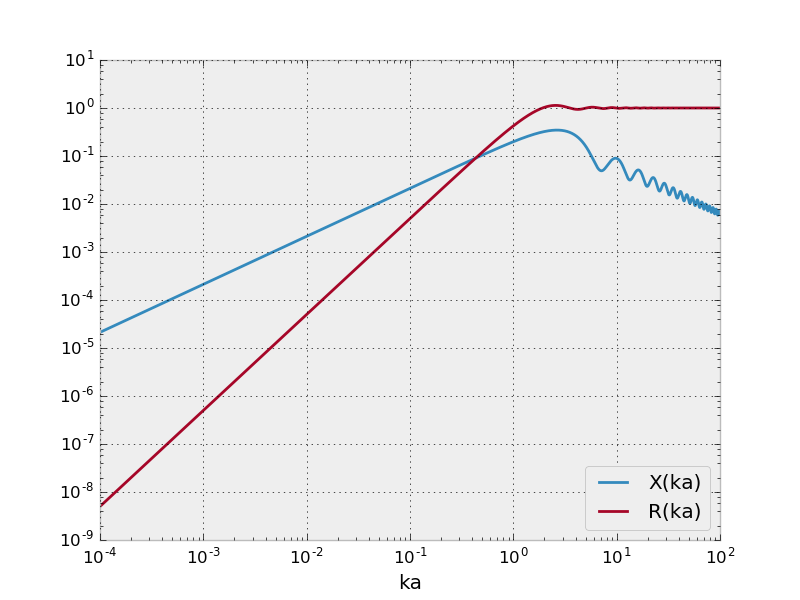
\includegraphics[width=\linewidth]{impedance.png}
\label{fig:impedance}
\caption{A log-log plot of the reactive and resistive parts of the mouth impedance in units such that $\rho c = 1$. At very low frequencies it can be seen that the impedance becomes primarily reactive and approaches a conservative system. At very high frequencies it becomes primarily resistive. In this regimes, its main effect will be to dissipate energy}
\end{figure}
\subsection{An Example}
Now that we have an expression for the mouth impedance we can solve the boundary value problem determined by Eqs. \ref{eq:helmholtz} and \ref{eq:boundary_two}. However first we should acknowledge that the real parts of $s$ and $Z$ make this boundary value problem non hermitian. The non hermitian nature of this boundary value problem reflects the presence of radiation from the mouth. This results in complex eigenvalues and non-orthogonal eigenfunctions. For a physically realistic treatment of the rat vocal tract we cannot ignore radiation from the mouth. We will deal with the difficulties of including this mechanism in a later chapter. In this section, as a simpler example, we will consider the boundary value problem in the low frequency approximation. This reduces to a hermitian problem and is an important historical result in acoustics. The low frequency approximation of $Z(\omega)$ can be derived by assuming the quantity $ka \ll 1$. In this limit we can expand Eq. \ref{eq:mouth_impedance} in powers of $ka$ and retain only linear terms. The impedance becomes
\begin{equation}
Z(\omega) \approx i \rho c  \frac{2 k a}{3\pi}.
\end{equation}
Here the resistive part of the impedance has become negligible, and the reactive part only provides a linear contribution. Substituting this into Eq. \ref{eq:boundary_two}, the boundary conditions becomes
\begin{equation}
\label{eq:low_frequency_impedance}
s_m \hat{\phi}_m(L, s_m) + c \frac{2ka}{3\pi} \frac{\partial }{\partial x}\hat{\phi}_m(L, s_m)= 0.
\end{equation}
Now solving Eq. \ref{eq:helmholtz} and applying the boundary condition at $x=0$ the eigenfunctions of the problem (up to a constant factor) are 
\begin{equation}
\label{eq:resonance_modes}
\hat{\phi}_m(x)= \sinh \left(\frac{s_m x}{c} \right)
\end{equation}
Plugging the expression functions into Eq. \ref{eq:low_frequency_impedance} we can get the characteristic equation, which determines the eigenvalues
\begin{equation}
\label{eq:characteristic1}
\tanh \left( \frac{s_m L}{c} \right) = -i \frac{2 k_m a}{3 \pi}.
\end{equation}
The real part of this equation is
\begin{equation}
\sinh \left(\frac{2 \alpha_m L}{c} \right) = 0. 
\end{equation}
This equation is only satisfied for $\alpha_m=0$, which indicates energy is not dissipated from the pipe due to radiation and that the problem is hermitian. With $\alpha_m=0$ Eq. \ref{eq:characteristic1} becomes 
\begin{equation}
\label{eq:characteristic}
\tan \left( k_m L \right) + \frac{2 k_m a}{3 \pi} = 0.
\end{equation}
This equation can be numerically solved for the eigenfrequencies. However, it is also instructive to expand the tan function out in a power series about its roots $m \pi$. Retaining only the linear term of the power series,
\begin{equation}
\label{eq:end_correction}
k_m \left( L + \frac{2 a}{3 \pi} \right) = m \pi.
\end{equation}
This is the same characteristic equation that is obtained from using the boundary condition $\hat{\phi}_m(L + \Delta L) = 0$ with $\Delta L = \frac{2 a}{3 \pi}$. The quantity $\Delta L$ is known as the end correction. So the additional reactance at the end of the pipe makes the resonance modes behave in the same way as if we use a zero stress boundary condition for a piple of length $L + \Delta L$. The interpretation of this is that in addition to the oscillations of the air inside the resonator there is a small amount of air that lies directly beyond that mouth that also oscillates. The inertia of this air must be taken into account when computing the resonance frequencies of the system. Fig. \ref{fig:end_correction} shows a plot of the characteristic equation and eigenfrequencies obtained using the end correction approximation. Fig. \ref{fig:resonance_modes} shows a plot of the resonance modes given by Eq. \ref{eq:resonance_modes}. This is often the stopping point of classical acoustics. However, an important question for our work is how does an acoustic system switch between the different resonance modes. It is my belief that the frequency jumps of rat ultrasonic vocalizations are the result of these kinds of transition. The frequency domain analysis is insufficient to answer to this question. In a later chapter we will go about formulating this problem in the time domain.
\begin{figure}
\centering
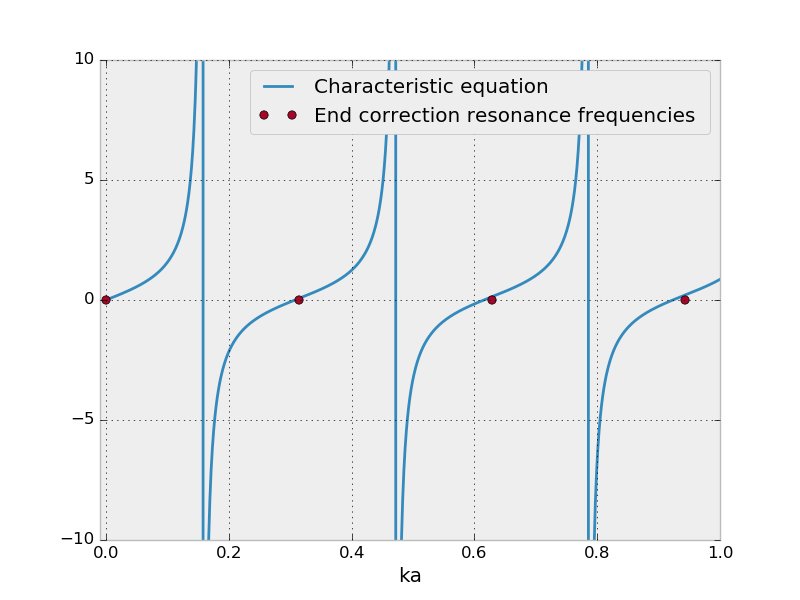
\includegraphics[width=\linewidth]{resonance_freqs.png}
\label{fig:end_correction}
\caption{A plot of the left hand side of Eq. \ref{eq:characteristic}for $L=10$ m and $a=1$ m. The roots of this function give the eigenfrequencies and can be approximated in the low frequency limit by Eq. \ref{eq:end_correction}, which is to equivalent to finding the eigenfrequencies of the system using the boundary condition $\hat{\phi}_m(L + \Delta L) = 0$. It can be seen that the end correction approximation starts to deviate from the true roots of the systems as $ka$ gets bigger. }
\end{figure}
\begin{figure}
\centering
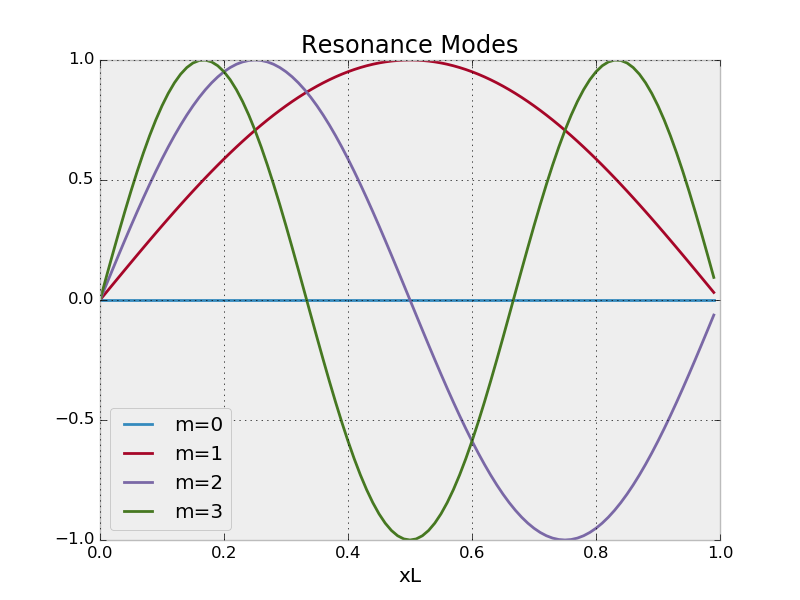
\includegraphics[width=\linewidth]{resonance_modes.png}
\label{fig:resonance_modes}
\caption{A plot of the left hand side of Eq. \ref{eq:characteristic}for $L=10$ m and $a=1$ m. The roots of this function give the eigenfrequencies and can be approximated in the low frequency limit by Eq. \ref{eq:end_correction}, which is to equivalent to finding the eigenfrequencies of the system using the boundary condition $\hat{\phi}_m(L + \Delta L) = 0$. It can be seen that the end correction approximation starts to deviate from the true roots of the systems as $ka$ gets bigger. }
\end{figure}

\section{Inviscid, Incompressible, Potential Flow}
\subsection{Bernoulli's Equation}
For this type of flow one simplifying assumption from the previous section will be relaxed and another simplifying assumption will be introduced. The flow will no longer be assumed to be linear, which was important in deriving the acoustic wave equation. However the inviscid and irrotational assumptions will be kept. These assumptions will allow the derivation of a conservation equation known as Bernoulli's equation. In addition it will be assumed the flow is incompressible, meaning variations in density can be neglected. This will simplify the continuity equation. In a later chapter we will use this type of flow to model the movement of air through the rat vocal folds throughout a vocalization. The relaxation of the linear assumption is important as it will allow us to take into account turbulent losses due to viscosity, even though we are analyzing the motion of an inviscid fluid. The incompressible assumption will simplify the continuity equation, which will allow us to analyze the flow without resorting to direct numerical simulations. In a previous section the equation of motion for an inviscid fluid was derived.
\begin{equation}
\rho \frac{D \textbf{v}}{D t} = -\nabla p.
\end{equation}
Writing out the convective derivative this becomes
\begin{equation}
\rho \left( \frac{\partial  \textbf{v}}{\partial t} +  (\textbf{v} \cdot \nabla)  \textbf{v} \right) = -\nabla p.
\end{equation}
Now we use the vector identity $(\textbf{v} \cdot \nabla)  \textbf{v}=\frac{1}{2} \nabla ( \textbf{v} \cdot \textbf{v} )$ to write the Euler equation as
\begin{equation}
\rho \left( \frac{\partial  \textbf{v}}{\partial t} +  \frac{1}{2} \nabla ( \textbf{v} \cdot \textbf{v} ) \right) = -\nabla p.
\end{equation}
Furthermore we can use the fact that the fluid is irrotational to write the velocity field as the gradient of a potential function $ \textbf{v} = \nabla \phi$. Substituting this into the above equation and factoring out the $\nabla$ operator we get
\begin{equation}
\nabla \left( \frac{\partial  \phi}{\partial t} +  \frac{1}{2}  \textbf{v} \cdot \textbf{v} + \frac{p}{\rho} \right) = 0.
\end{equation}
In this step we have used the fact that the fluid is incompressible, since we assumed $\rho$ is constant when we factored out the $\nabla$ operator. Now we can integrate this expression between any two points in the fluid. The curve connecting these two points is irrelevant, since the fluid is irrotational. It is only the end points that matter.
\begin{equation}
\int_1^2 d\textbf{s} \cdot \nabla \left( \frac{\partial  \phi}{\partial t} +  \frac{1}{2}  \textbf{v} \cdot \textbf{v} + \frac{p}{\rho} \right) = 0.
\end{equation}
Using the fundamental theorem of calculus we get Bernoulli's equation for an unsteady, inviscid, potential flow.
\begin{equation}
\frac{\partial  \phi_1}{\partial t} +  \frac{v_1^2}{2} + \frac{p_1}{\rho}=\frac{\partial  \phi_2}{\partial t} +  \frac{v_2^2}{2} + \frac{p_2}{\rho},
\end{equation}
where we have defined $v^2 = \textbf{v} \cdot \textbf{v}$. The interpretation of this equation is that quantity on either side is the same throughout all points in the fluid.

\subsection{The Continuity Equation}
Bernoulli's equation describes conservation of energy between any two points in an inviscid irrotational fluid. In practice a conservation of mass equation is also needed to fully determine the flow variables. We will eventually the rat vocal as a series of cylindrical pipes. For this physical configuration the incompressible continuity equation takes an especially simple form. If we neglect variations in density in Eq. \ref{eq:continuity}, we get the incompressible continuity equation
\begin{equation} 
\label{eq:incompressible}
\nabla \cdot \textbf{v}=0.
\end{equation}
Suppose we have two points $1$ and $2$, separated by an axial distance in a cylindrical pipe of varying area. The area of the pipe at point $1$ is $A_1$, and the area of the pipe at point $2$ is $A_2$. Integrating Eq. \ref{eq:incompressible} over the volume $V$ of the pipe bounded by areas $A_1$ and $A_2$
\begin{equation} 
\int_V dV \nabla \cdot \textbf{v}=0.
\end{equation}
Now we can use the divergence theorem to write this integral as a surface integral over the surface area $A$ of $V$.
\begin{equation} 
\int_A d\textbf{A} \cdot \textbf{v}=0.
\end{equation}
Now because of the zero penetration condition (i.e. there can not be any fluid flowing into the walls of the pipe) the quantity $d\textbf{A} \cdot \textbf{v}=0$ on the walls of the pipe. So the above integral reduces to the sum of surface integrals over $A_1$ and $A_2$.
\begin{equation} 
\int_{A_1} d\textbf{A} \cdot \textbf{v}_1 + \int_{A_2} d\textbf{A} \cdot \textbf{v}_2=0.
\end{equation}
This equation states that the volume flow of fluid through surface $A_1$ must be balanced out by the flow of fluid through surface $A_2$. If we assume the fluid flows through the pipe in one direction (say from $1$ to $2$). Further we can assume that flow velocity only varies axially, not radially or azimuthally, then the quantity $d\textbf{A} \cdot \textbf{v}$ is constant on $A_1$ and $A_2$, and we can write
\begin{equation} 
A_1 \textbf{v}_1 \cdot \textbf{n}_1 + A_2 \textbf{v}_2 \cdot \textbf{n}_2 =0,
\end{equation}
where $\textbf{n}_1$ and $\textbf{n}_2$ are the outward normal vectors for surfaces $A_1$ an $A_2$. If we further assume the flow is axial, this simplifies even further.
\begin{equation}
A_1 v_1 = A_2 v_2.
\end{equation}
This continuity equation for axial incompressible pipe flow. We will later use it in our analysis of the flow through the rat vocal folds.

\section{Nonlinear Energy Losses at an Orifice}
In this section we will use Bernoulli's equation to analyze the energy losses of a fluid as it flows through a circular aperture of area $A_f$ and length $L$. In a later chapter we will use the results from this section to model the flow of air through the rat vocal folds. Let's consider two points directly before and after the start of the aperture. We'll call these points $1$ and $2$. The pressure at those points is $p_1$ and $p_2$ respectively. Now as first approximation, let's consider the air in the circular aperture as an incompressible cylindrical slug, being accelerated by the pressure difference $\Delta p = p_2 - p_1$. From Newton's second law the time rate of change of the velocity of the slug is 
\begin{equation}  
\label{eq:linear_aperture}
\rho_0 L A_f \dot{u}_f = p_1 A_f - p_2 A_f = -\Delta p A_f,
\end{equation}
where $\rho_0 L A_f$ is the mass of the air in the aperture and $u_f$ is its velocity (we are using the subscript $f$ for these quantities because we later use this analysis to model the flow through the vocal folds). If we force the slug of air with a sinusoidal pressure difference of the form
\begin{equation}
\Delta p = |p| \cos{\omega t},
\end{equation}
the velocity of the slug of air can be calculated with Eq. \ref{eq:linear_aperture}.
\begin{equation}
u_f = -\frac{|p|}{\rho_0 L \omega} \sin{omega t}.  
\end{equation}
Thus, the amplitude of the velocity oscillations is $\frac{|p|}{\rho_0 L \omega}$. This is exactly the relationship Ingard and Ising measured for low velocity flows through a circular orifice. They found as long as the velocities were below a threshold value value the, the relationship between pressure and velocity amplitudes was linear. However, they found something somewhat surprising. For velocities greater than that threshold value the relationship became quadratic \cite{Ingard1967}. Our above analysis does not predict this relationship because in calculating the relationship between pressure and velocity amplitudes we neglected the formation of the air into a jet. This jet has kinetic energy associated with it, which is lost due to turbulent dissipation when the jet expands outward on the other side of the orifice. We can use Bernoulli's equation to calculate this nonlinear energy loss. Writing down Bernoulli's Equation between points $1$ and $2$, where we assume the assume the air flowing through the aperture has already formed into a jet with velocity $u_f$ at point $1$. Furthermore, we also assume at point $2$ the kinetic energy has been completely dissipated due to turbulence.
\begin{equation}  
\Delta_p - \frac{\rho_0}{2} u_f^2 + \rho_0 \frac{\partial }{\partial t}\left( \phi_2 - \phi_1  \right) = 0.
\end{equation}
The velocity potential difference is related to the velocity of the air in the aperture $u(x)$ through the equation $\phi_2 - \phi_1 = \int_1^2 u(x) dx$. As long as the radius of the aperture is constant we can approximate the velocity of the air in the aperture as constant and the potential difference can be written as $\phi_2 - \phi_1 = u_f L$. The energy balance equation becomes 
\begin{equation}  
\label{eq:nonlinear_aperture}
\delta_p - \frac{\rho_0}{2} u_f^2 + \rho_0 L \dot{u}_f = 0.
\end{equation}
This equation gives the quadratic relationship, observed by Ingard and Ising, between the pressure drop across the orifice and the velocity of flow through the orifice. Furthermore, it reduces to Eq. \ref{eq:linear_aperture} for low values of $u_f$. This result is actually quite interesting. Even though we assumed inviscid and irrotational flow through the aperture we obtained an expression for the nonlinear energy losses due to viscous turbulent dissipation. The relevance of this result will become more apparent in a later chapter when we use the pressure on the far side of the aperture to model the driving of resonance modes in the upper vocal tract of the rat. The nonlinear energy losses will serve to keep the time domain simulations bounded.  

\bibliography{mdornfe1.bib}
\end{document} 